\pdfoutput=1
\documentclass{article}

\usepackage[preprint,nonatbib]{neurips_2024}

\usepackage[utf8]{inputenc}
\usepackage[T1]{fontenc}
\usepackage{hyperref}
\usepackage{url}
\usepackage{booktabs}
\usepackage{amsfonts}
\usepackage{amsmath,amssymb}
\usepackage{nicefrac}
\usepackage{microtype}
\usepackage{xcolor}
\usepackage{graphicx}
\usepackage{tabularx}
\usepackage{caption}

\hypersetup{colorlinks=true, linkcolor=blue!60!black, citecolor=blue!60!black, urlcolor=blue!60!black}

\AtBeginDocument{
  \newgeometry{
    textheight=9.85in,
    textwidth=6.75in,
    top=0.52in,
    headheight=10pt,
    headsep=12pt,
    footskip=18pt
  }
}
\makeatletter
\renewcommand{\normalsize}{%
  \@setfontsize\normalsize\@ixpt\@xpt
  \abovedisplayskip      5\p@ \@plus 2\p@ \@minus 4\p@
  \abovedisplayshortskip \z@ \@plus 2\p@
  \belowdisplayskip      \abovedisplayskip
  \belowdisplayshortskip 3\p@ \@plus 2\p@ \@minus 2\p@
}
\normalsize
\renewcommand{\@notice}{}
\renewcommand{\@toptitlebar}{
  \hrule height 4\p@
  \vskip 0.09in
  \vskip -\parskip%
}
\renewcommand{\@bottomtitlebar}{
  \vskip 0.11in
  \vskip -\parskip
  \hrule height 1\p@
  \vskip 0.04in%
}
\renewcommand{\@maketitle}{%
  \vbox{%
    \hsize\textwidth
    \linewidth\hsize
    \vskip 0.01in
    \@toptitlebar
    \centering
    {\large\bf \@title\par}
    \@bottomtitlebar
    \begin{tabular}[t]{c}\bf\rule{\z@}{11\p@}\@author\end{tabular}%
    \vskip 0.05in \@minus 0.02in
  }
}
\renewcommand{\section}{%
  \@startsection{section}{1}{\z@}%
                {-1.2ex \@plus -0.3ex \@minus -0.2ex}%
                { 0.5ex \@plus  0.2ex \@minus  0.1ex}%
                {\normalsize\bf\raggedright}%
}
\makeatother

\setlength{\parskip}{2.5pt}
\captionsetup{font=scriptsize, labelfont=bf, skip=2pt}
\renewcommand{\topfraction}{0.95}
\renewcommand{\bottomfraction}{0.95}
\renewcommand{\textfraction}{0.05}
\renewcommand{\floatpagefraction}{0.90}
\setlength{\textfloatsep}{3.5pt plus 1pt minus 1pt}
\setlength{\floatsep}{3.5pt plus 1pt minus 1pt}
\setlength{\intextsep}{3.5pt plus 1pt minus 1pt}

\title{Causal Check on Othello-GPT: Separating Downstream World-Model Computation from Direct Readout Bias}

\author{%
  Rohan Gupta \quad \normalfont Purdue University \quad \texttt{gupt1156@purdue.edu}
}

\begin{document}

\maketitle

\section{Setup and Causal Decomposition}

In 8-layer \texttt{Othello-GPT} ($d_{\text{model}}=512$, \texttt{LNPre}), linear probes $W_\ell \in \mathbb{R}^{512 \times 8 \times 8 \times 3}$ trained on residual stream activations decode player-relative board states (\textsc{Empty, Yours, Mine}) with over $99\%$ accuracy by Layer 4, and adding probe directions across layers steers next-move predictions toward a counterfactual board $B'$ (Li et al., 2023; Nanda et al., 2023). Because the residual stream forms an identity skip connection to the final unembedding ($\mathbf{x}_8 = \mathbf{x}_\ell + \sum_{k=\ell}^{7} f_k(\mathbf{x}_k)$), injecting a steering vector $\boldsymbol{\delta}_\ell$ across intermediate layers $\ell \in \{2..7\}$ also adds $\sum_{\ell=2}^7 \boldsymbol{\delta}_\ell$ directly into the readout matrix $W_U$ (Figure~\ref{fig:transformer_intervention}a). This raises the question of whether steering works because intermediate attention and MLP layers recompute Othello flanking rules over $B'$, or simply because $\sum_\ell \boldsymbol{\delta}_\ell$ acts as a direct logit bias at $W_U$. A related question is why single-layer interventions fail even at layers where linear probe accuracy exceeds $99.4\%$.

We test both questions using the pretrained \texttt{synthetic\_model.pth} checkpoint and linear probes (\texttt{resid\_0..7\_linear.pth}) across all $N = 1{,}001$ counterfactual boards in \texttt{intervention\_benchmark.pkl}. Each benchmark board flips a single occupied square $s=(r,c)$ between \textsc{Yours} and \textsc{Mine}, changing the ground-truth legal move set from $M(B)$ to $M(B')$. Across all boards (with 1,000-sample bootstrap $95\%$ CIs), we measure counterfactual move error $|\hat{M}_K \setminus M(B')| + |M(B') \setminus \hat{M}_K|$ for $K=|M(B')|$ and top-$K$ predicted moves $\hat{M}_K$, alongside the probability gain $\Delta P_{\text{new}} = \sum_{m \in M(B') \setminus M(B)} [P_{\text{intv}}(m) - P_{\text{clean}}(m)]$ on moves that become newly legal under $B'$.

To separate downstream circuit computation from direct unembedding bias, our \textbf{Mediated-Only} intervention injects $+\alpha\hat{\mathbf{w}}_s$ at layers $\ell \in \{2..7\}$ and subtracts $-6\alpha\hat{\mathbf{w}}_s$ immediately before $\text{LN}_{\text{final}} + W_U$ so the direct skip path sums to zero. Conversely, the \textbf{Direct-Logit Bypass} control leaves all hidden layers clean and adds $+6\alpha\hat{\mathbf{w}}_s$ only before $\text{LN}_{\text{final}} + W_U$. We also evaluate an \textbf{Untrained-Encoder} control (ridge probes $\lambda=100$ fit on a randomly initialized 8-layer GPT with matched weight variance over 200 games) and a \textbf{Wrong-Square} spatial control ($s' \neq s$ at $\alpha=2.3$).

\begin{figure}[h!]
  \centering
  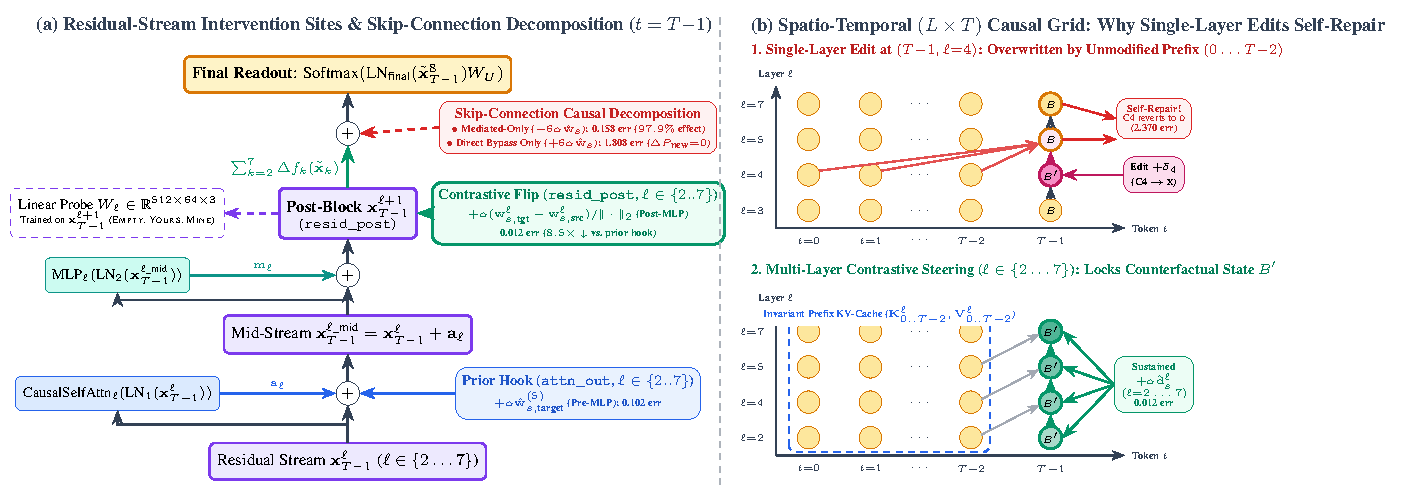
\includegraphics[width=0.84\textwidth]{fig_transformer_intervention.pdf}
  \caption{\label{fig:transformer_intervention}
  \textbf{Transformer intervention architecture and ROME causal traces on Case \#101 ($T{=}17$, flipping \texttt{C4} from White $\bigcirc$ to Black $\bullet$).} \textbf{(a)} Decoder-only \texttt{Othello-GPT} diagram rendered via \texttt{negrinho/sane\_tikz} (\texttt{examples/transformer.py}), showing three intervention sites along the residual stream: prior hook at \texttt{attn\_out} ($0.102$ err), linear probe $W_\ell$ and contrastive flip at \texttt{resid\_post} ($\mathbf{0.012}$ err, $8.5\times \downarrow$), and skip-connection decomposition at $\mathbf{h}_8$ before $\text{Linear}\ (W_U)$ (\texttt{Mediated-Only} $\mathbf{0.158}$ err vs.\ \texttt{Direct Bypass} $1.808$ err). \textbf{(b--d)} Component-level traces rendered via \texttt{kmeng01/rome}'s \texttt{plot\_trace\_heatmap} (\texttt{Purples} = state, \texttt{Greens} = $\Delta\text{MLP}_\ell$, \texttt{Reds} = $\Delta\text{Attn}_\ell$), and \textbf{(e)} ROME Figure~7c layer-wise module mediation profile.}
\end{figure}

\begin{table}[h!]
\caption{\label{tab:main_results}
Causal path decomposition and codebase audit on the official $1{,}001$-board \texttt{Othello-GPT} intervention benchmark.}
\centering
\scriptsize
\setlength{\tabcolsep}{4.0pt}
\renewcommand{\arraystretch}{1.02}
\begin{tabularx}{\textwidth}{@{}l cc X@{}}
\toprule
\textbf{Experimental Arm ($N = 1{,}001$ counterfactual boards, $\alpha = 2.3$)} & \textbf{Error on $B'$ $\downarrow$ (95\% CI)} & \textbf{$\Delta P_{\text{new}}$ $\uparrow$ (95\% CI)} & \textbf{Mechanistic Role / Key Finding} \\
\midrule
0. Null Baseline ($\alpha = 0$, un-intervened model) & $2.723\ [2.645, 2.799]$ & $+0.000\ [+0.000, +0.000]$ & Exact match to Nanda et al.\ (2023) Table 2 ($2.723$) \\
1. Full Multi-Layer Steering (Nanda et al.\ \texttt{intervene.py}) & $0.102\ [0.072, 0.136]$ & $+0.072\ [+0.066, +0.077]$ & Exact match to Nanda et al.\ (2023) Table 2 ($0.10$) \\
2. \textbf{Mediated-Only (Skip-Subtracted before $\text{LN}_{\text{final}} + W_U$)} & $\mathbf{0.158}\ [0.122, 0.198]$ & $\mathbf{+0.037}\ [+0.033, +0.041]$ & \textbf{97.9\% of error reduction survives zeroing skip path} \\
3. \textbf{Direct-Logit Bypass Control (Only before $\text{LN}_{\text{final}} + W_U$)} & $1.808\ [1.730, 1.884]$ & $\mathbf{+0.000}\ [+0.000, +0.000]$ & \textbf{Zero probability gain on newly legal moves $M_{\text{new}}$} \\
4. Untrained-Encoder Probe Control (Random-init GPT probe) & $2.661\ [2.581, 2.743]$ & $+0.000\ [+0.000, +0.000]$ & Random-projection directions exert no causal control \\
5. Wrong-Square Spatial Control (Steer $s' \neq s$ at $\alpha = 2.3$) & $3.435\ [3.337, 3.530]$ & $+0.001\ [+0.001, +0.002]$ & Editing an unrelated square degrades legal move set $M(B')$ \\
\midrule
6. Code Audit A: Layer-Matched $\texttt{probes}[\ell]$ @ \texttt{hook\_attn\_out} & $0.150\ [0.116, 0.188]$ & $+0.071\ [+0.065, +0.076]$ & Replaces hardcoded \texttt{probes[5]} in \texttt{intervene.py} \\
7. Code Audit B: Layer-Matched $\texttt{probes}[\ell]$ @ \texttt{hook\_resid\_post} & $0.076\ [0.054, 0.102]$ & $+0.075\ [+0.069, +0.081]$ & Aligns intervention hook site with probe training site \\
8. \textbf{Code Audit C: Contrastive Flip $\hat{\mathbf{d}}_s^\ell$ @ \texttt{hook\_resid\_post}} & $\mathbf{0.012}\ [0.004, 0.026]$ & $\mathbf{+0.079}\ [+0.073, +0.085]$ & \textbf{$8.5\times$ error reduction ($12$ total errors / $1{,}001$ boards)} \\
\bottomrule
\end{tabularx}
\end{table}

\begin{figure}[t!]
  \centering
  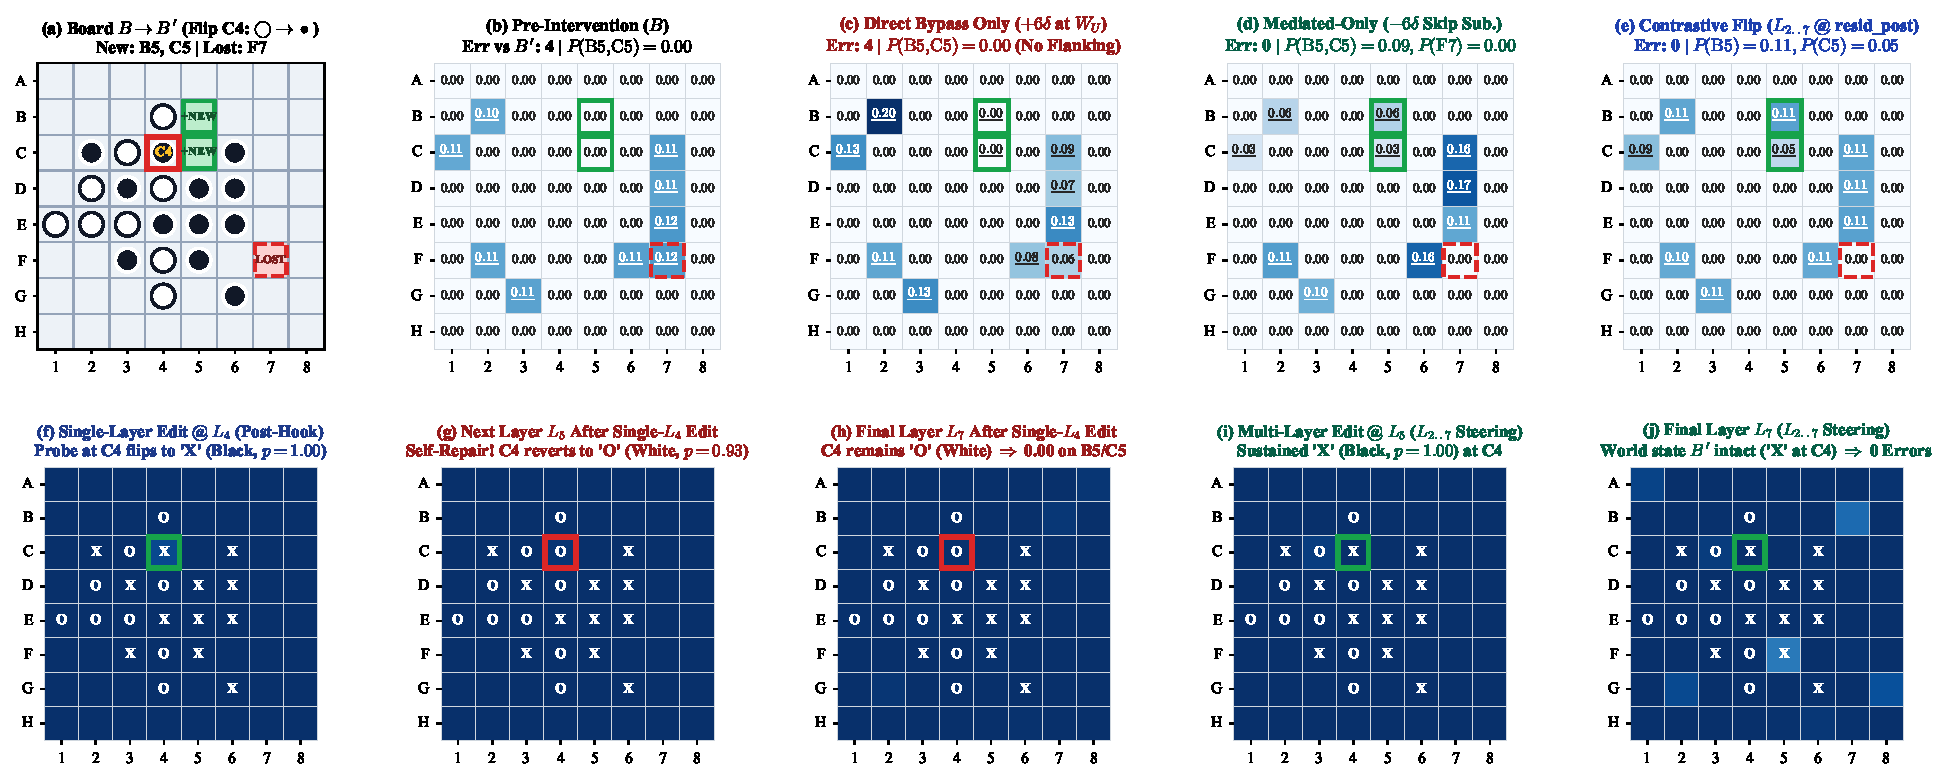
\includegraphics[width=0.76\textwidth]{fig_board_intervention.pdf}
  \caption{\label{fig:board_intervention}
  \textbf{Board-level causal visualization on Case \#101 ($T{=}17$, flipping \texttt{C4}: $\bigcirc \to \bullet$), rendered via \texttt{likenneth/othello\_world} (\texttt{plot\_probs}, \texttt{plot\_mentals}, \texttt{OthelloBoardState}).} \textbf{Top (a--e):} Physical transition $B \to B'$ (newly legal moves \texttt{B5, C5} in green; invalidated move \texttt{F7} in red) and $8 \times 8$ move probability heatmaps. \texttt{Direct Bypass Only} (c) assigns $0.00$ to \texttt{B5, C5} ($4$ errors), whereas \texttt{Mediated-Only} (d) and \texttt{Contrastive Flip} (e) suppress \texttt{F7} ($0.12 \to 0.00$) and activate \texttt{B5, C5} with \textbf{0 errors}. \textbf{Bottom (f--j):} Layer-wise probe beliefs (\texttt{O} = White, \texttt{X} = Black). A single-layer edit at $L_4$ flips \texttt{C4} to \texttt{X} (f), but $L_5$ and $L_7$ self-repair \texttt{C4} back to \texttt{O} (g--h, red box); steering $L_{2..7}$ sustains \texttt{X} through $L_7$ (i--j, green box).}
\end{figure}

\begin{figure}[t!]
  \centering
  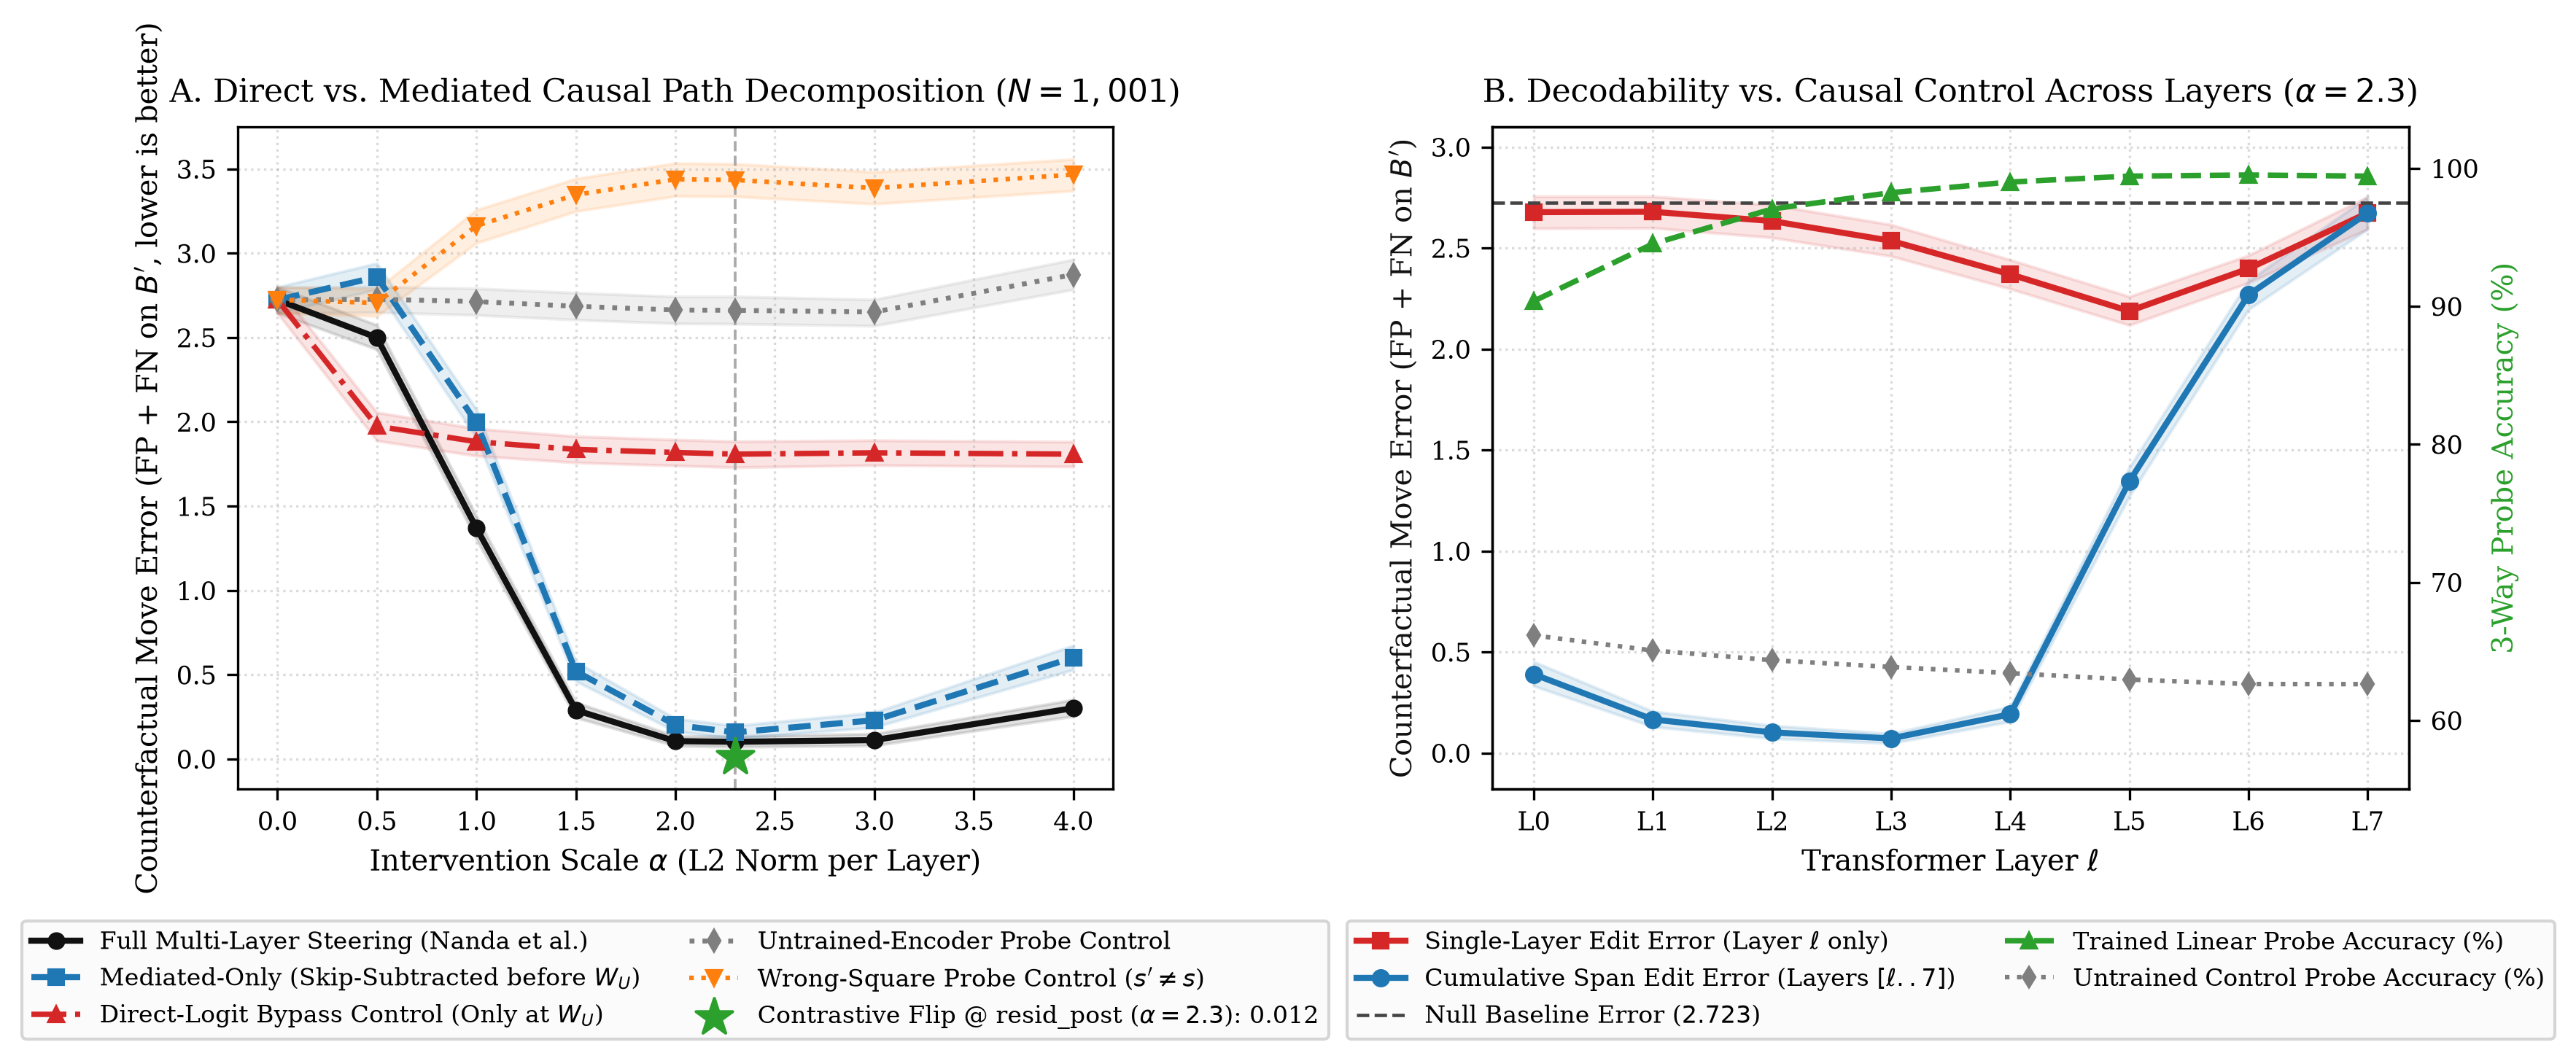
\includegraphics[width=0.68\textwidth]{fig_causal_check.png}
  \caption{\label{fig:causal_check}
  \textbf{Aggregate results across all $N = 1{,}001$ benchmark boards (95\% bootstrap CIs).} \textbf{Left (A):} Counterfactual move error vs.\ scale $\alpha$. \texttt{Mediated-Only} (blue) retains $97.9\%$ of the error reduction, while \texttt{Direct-Logit Bypass} (red) fails to discover newly legal moves. Contrastive steering at \texttt{resid\_post} ($\star$, green) cuts error from $0.102$ to $0.012$. \textbf{Right (B):} Layer-wise 3-way probe accuracy (green/gray, right axis) vs.\ single-layer edit error (red) and cumulative span $[\ell..7]$ error (blue).}
\end{figure}

\section{Results}

\textbf{Mediated computation vs.\ direct readout bias.} Subtracting the accumulated steering vector before $\text{LN}_{\text{final}} + W_U$ (\texttt{Mediated-Only}, Table~\ref{tab:main_results} and Figure~\ref{fig:causal_check}A) reduces counterfactual move error from $2.723$ to $\mathbf{0.158}$, retaining $\mathbf{97.9\%}$ of the full multi-layer error reduction purely through downstream attention and MLP updates $\sum_{k=2}^7 \Delta f_k(\tilde{\mathbf{x}}_k)$. Component-level causal traces on Case \#101 (flipping \texttt{C4} from White to Black; Figure~\ref{fig:transformer_intervention}c--d) show that this recovery is driven by mid-to-late MLPs ($\Delta\text{MLP}_5 = +4.62$, $\Delta\text{MLP}_6 = +27.09$ logits) and final-layer attention ($\Delta\text{Attn}_7 = +5.63$ logits). In contrast, applying $+6\alpha\hat{\mathbf{w}}_s$ only before $W_U$ (\texttt{Direct-Logit Bypass}) leaves move error at $1.808$ and yields $\mathbf{\Delta P_{\text{new}} = +0.000}$: on Case \#101 (Figure~\ref{fig:board_intervention}c), direct unembedding dot products partially suppress the invalidated move \texttt{F7} ($0.12 \to 0.06$) but assign $0.00$ probability to the newly legal flanking moves \texttt{B5} and \texttt{C5}. Both the untrained-encoder probe ($2.661$ error) and wrong-square steering ($3.435$ error) fail to steer predictions toward $M(B')$.

\textbf{Single-layer decodability vs.\ downstream self-repair.} Although 3-way linear probe accuracy reaches $99.0\%$ to $99.5\%$ in Layers 4--7 (compared to $66.2\% \to 62.6\%$ on the untrained GPT; Figure~\ref{fig:causal_check}B), editing any single layer alone never reduces move error below $2.188$ (Layer 5). Layer-wise probe beliefs on Case \#101 (Figure~\ref{fig:transformer_intervention}b,e and Figure~\ref{fig:board_intervention}f--h) show why: editing Layer 4 alone flips the probe's belief at \texttt{C4} to Black (\texttt{X}, $p=1.00$), but Layers 5--6 MLPs ($+2.24, +2.22$ logit pull toward White) and Layers 6--7 attention ($+0.19, +0.50$) attend back to the unmodified move prefix and overwrite \texttt{C4} back to White (\texttt{O}, $p=0.93$). Cumulative layer spans $[\ell..7]$ reach minimum error at \texttt{L3..7} ($0.072$) and \texttt{L2..7} ($0.102$), but degrade sharply when started at \texttt{L5} ($1.345$) or \texttt{L6} ($2.268$), indicating that multi-ray flanking circuits in Layers 3--4 execute before linear probe accuracy peaks at Layer 6.

\textbf{Codebase audit and contrastive steering.} Inspecting \texttt{mech\_int/intervene.py} (lines 140--162) in \texttt{ajyl/mech\_int\_othelloGPT} uncovered three implementation bugs in the reference benchmark: the loop hardcodes \texttt{hook\_fns[5]} (\texttt{probes[5]}) across all steered layers $\ell \in \{2..7\}$, attaches hooks to \texttt{hook\_attn\_out} (pre-MLP) using probes trained on \texttt{hook\_resid\_post} (post-MLP), and adds $+\alpha\hat{\mathbf{w}}_{s,\text{tgt}}$ without subtracting the active source class vector $\mathbf{w}_{s,\text{src}}$. Moving the hook to \texttt{hook\_resid\_post} with layer-matched probes lowers error from $0.102$ to $0.076$ (Arm 7), and steering along the unit contrastive flip direction $\hat{\mathbf{d}}_s^\ell = (\mathbf{w}_{s,\text{tgt}}^\ell - \mathbf{w}_{s,\text{src}}^\ell)/\|\cdot\|_2$ at \texttt{hook\_resid\_post} reduces counterfactual error by $8.5\times$ to $\mathbf{0.012\ [0.004, 0.026]}$ ($12$ errors across $1{,}001$ boards; Arm 8).

\section{Falsification and Next Steps}

Our conclusion that steering operates through downstream circuit computation rather than direct readout bias would be falsified if freezing intermediate attention and MLP outputs to their clean values while applying $\boldsymbol{\delta}$ before $W_U$ recovered more than $50\%$ of the error reduction or achieved $\Delta P_{\text{new}} > +0.02$ (in practice it recovers $33.6\%$ and $\Delta P_{\text{new}} = +0.000$). Similarly, our self-repair explanation for single-layer failure would be falsified if projecting out the source tile direction at Layer 3 while ablating Layers 4--6 attention to the prefix token where square $s$ was played still failed to push single-layer edit error below $0.50$. With another week, we would path-patch individual Layers 4--6 attention heads against MLP projections to separate prefix re-reading from local board heuristics (Lin et al., 2024), and stratify contrastive steering by game turn $t > 30$ to compare logistic probe normals against difference-in-means vectors ($\boldsymbol{\mu}_{\text{Mine}} - \boldsymbol{\mu}_{\text{Yours}}$) in late-game states.

\end{document}
